\chapter{Future Work}
\label{c.future}

\section{Eigenspectrum Characterization for Signal Loss}

In Chapter \ref{c.PSmethods}, we discussed how weighting data by an empirical covariance can lead to overfitting of the cosmological signal, resulting in signal loss in a 21\,cm power spectrum. We investigated the relationship between an empirical covariance (namely, its convergence to the true covariance) and the number of independent samples in a data set, and we found, as expected, that convergence rates are fastest when averaging over large numbers of data realizations (Figure \ref{fig:toy_sigloss16}). Additionally, we began to explore the relationship between eigenvector convergence and the shape of an eigenspectrum, finding that steep eigenspectra (with eigenmodes that have eigenvalues that differ greatly from each other) converge the fastest (Figure \ref{fig:toy_sigloss17}).

In this section, we expand our preliminary analysis characterizing covariance eigenspectra and outline future work on this topic. Ideally, we would like to define a metric that relates an eigenspectrum to the amount of potential signal loss it will incur when weighting by it. This would be useful because it would provide a method to estimate, \textit{a priori}, how much signal loss may result given a particular covariance. To define this metric, we must understand how different properties of an eigenspectrum, including its shape and its error bars, affect its convergence. 

Let's first begin by looking at the rate of convergence of empirical eigenvectors to their true forms. In Chapter \ref{sec:toymodel_frf} we described how eigenvectors of an empirical covariance are strongly coupled to the data (which leads to loss), and the rate at which they can effectively "un-couple" and approach their true shapes affects how much signal loss results. A steep eigenspectrum, where each eigenmode has a distinct eigenvalue, can more easily de-tangle its eigenvectors, whereas a flat eigenspectrum contains many degenerate eigenvectors and thus requires many more data realizations to "un-do" the coupling. 

To quantify this effect, we simulate a noise-like EoR signal similarly to Chapter \ref{sec:toymodel_frf}, where we construct a covariance whose true form is a diagonal matrix in the Fourier domain with eigenvalues spanning some range. The Fourier-transform of this covariance is the covariance of the EoR in the frequency domain, or $\textbf{C}_{\rm EoR}$. For different numbers of realizations, we draw random EoR signals that are consistent with $\textbf{C}_{\rm EoR}$ and compute the combined empirical covariance by averaging over the realizations. On the vertical axis of Figure \ref{fig:eigchar_1}, we plot a convergence metric that describes the covariance's empirical eigenvectors $\widehat{\textbf{v}}$ compared to the true eigenvectors $\textbf{v}$, namely Equation \eqref{eq:converge_eig}, or:

\begin{equation}
\label{eq:converge_eig2}
\varepsilon (\widehat{\textbf{v}}) \equiv \sqrt{\sum_{i}^{N_{f}}|\textbf{v}-\widehat{\textbf{v}}|_{i}^2},
\end{equation}
where small $\varepsilon (\widehat{\textbf{v}})$ denotes faster convergence.

We run this simulation over a range of realizations and for true covariances whose eigenvalues range from a span of one order of magnitude to five (i.e., a relatively flat spectrum to steep). Most importantly, the horizontal axis of Figure \ref{fig:eigchar_1} captures two important properties of an eigenspectrum that we would like to relate to convergence: uncertainty (errors) of the spectrum, and relative slope of the spectrum. The reason we choose to look at these two properties is because together they describe how much "overlap" there is between eigenmodes. More overlap (i.e., a flat spectrum and/or large errors) means that it is more difficult for the empirical eigenvectors to de-couple from each other, slowing convergence. 

In practice, the eigenvalue errors in our simulation come from the distribution of empirical eigenvalues obtained from running $N$ total simulations, where $N$ is large. The quantity we then form for every $i^{th}$ eigenmode (except the smallest one, when ordered from largest to smallest) is a fractional error (FE):

\begin{equation}
FE = \frac{\sigma_{i} + \sigma_{i+1}}{2(\lambda_{i} - \lambda_{i+1})},
\end{equation}
where $\sigma$ are eigenvalue errors and $\lambda$ are eigenvalues. This quantity thus captures both how much overlap there is between eigenvalues (the numerator, or average of two adjacent errors) and how steep the spectrum is (the denominator). 

\begin{figure}
    \centering
	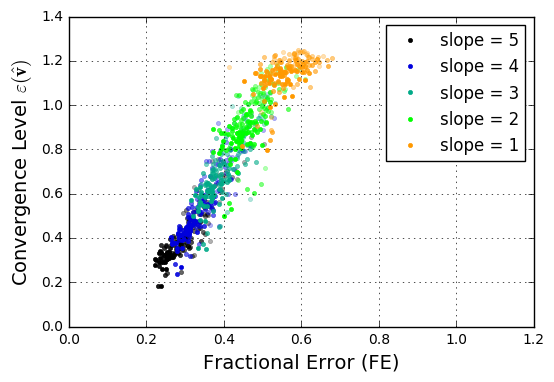
\includegraphics[width=0.65\textwidth]{plots/eigchar_1.png}    
	\caption{The convergence level (y-axis), as defined by Equation \eqref{eq:converge_eig2}, of empirically estimated eigenvectors compared a fractional error metric of the eigenspectrum (x-axis) which takes into account both how well-defined and how steep the spectrum is. The different colors denote the number of orders of magnitude that the true eigenspectrum spans. It appears that the defined fractional error quantity is closely related to eigenvector convergence, with smaller errors and steeper spectrum slopes converging fastest.}
    \label{fig:eigchar_1}
\end{figure}

\begin{figure}
    \centering
	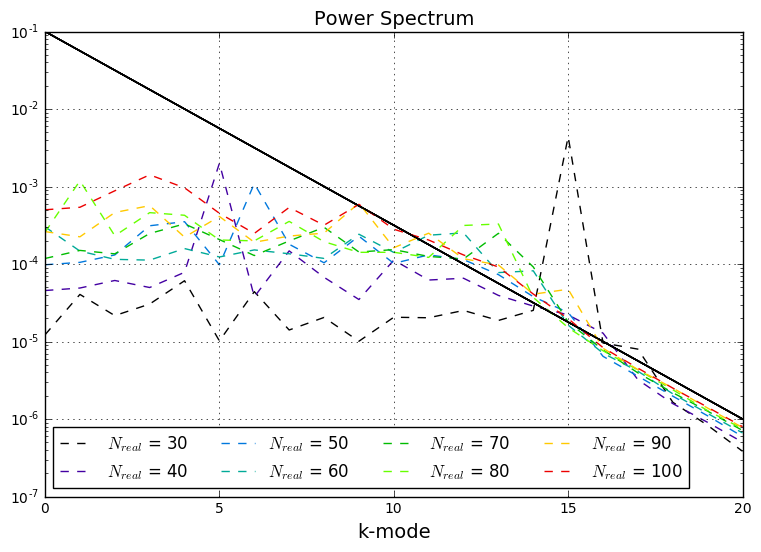
\includegraphics[width=0.65\textwidth]{plots/eigchar_2.png}    
	\caption{Resulting power spectra for different numbers of realizations (dashed colors) compared to the true power spectrum (solid black), which spans five orders of magnitude. Although increasing the number of realizations decreases loss as expected, there is still obvious signal loss at low $k$-modes.}
    \label{fig:eigchar_2}
\end{figure}

\begin{figure}
    \centering
	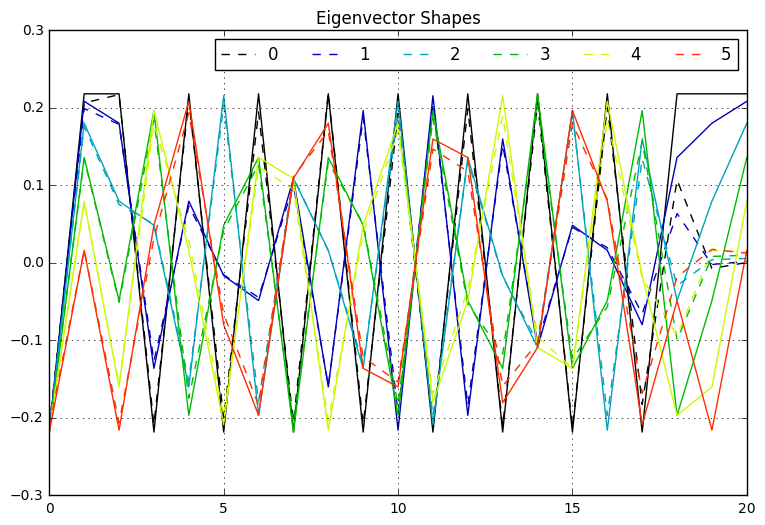
\includegraphics[width=0.65\textwidth]{plots/eigchar_3.png}    
	\caption{Eigenvector shapes for a few of the first modes (different colors) for the simulation corresponding to $N_{real}=100$ in Figure \ref{fig:eigchar_2}. The empirical eigenvectors (dashed) are in general converged to their true forms (solid), implying that there should be minimal signal loss. However, we see significant signal loss in Figure \ref{fig:eigchar_2}.}
    \label{fig:eigchar_3}
\end{figure}

\begin{figure}
    \centering
	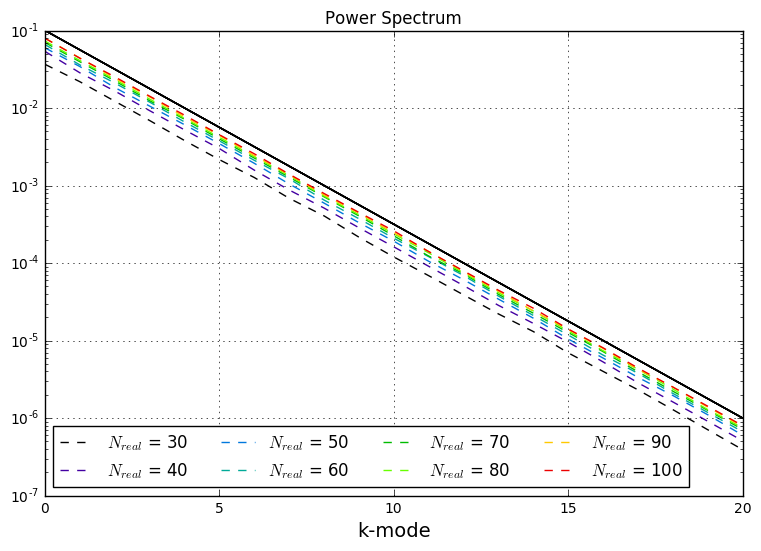
\includegraphics[width=0.65\textwidth]{plots/eigchar_4.png}    
	\caption{Resulting power spectra for different numbers of realizations (dashed colors) compared to the true power spectrum (solid black), which spans five orders of magnitude. This plot differs from Figure \ref{fig:eigchar_2} only in window function shapes; here our window functions are set to estimate power spectrum modes independently from each other. We find that by de-tangling window function modes, we avoid significant signal loss that results in Figure \ref{fig:eigchar_2} due to information from high $k$-modes dragging down low $k$-modes.}
    \label{fig:eigchar_4}
\end{figure}

From Figure \ref{fig:eigchar_1}, we see that the fractional error quantity we defined is closely related to eigenvector convergence, with eigenspectra with smaller errors converging fastest. Looking at the different colors, we also see that eigenspectra with steeper slopes converge fastest, which is in alignment with our discussion above. We have therefore showed how eigenvector convergence depends on properties of an eigenspectrum, and our next step is to relate convergence to signal loss. 

Up until now, we have implied that a converged covariance (and more specifically, converged eigenvectors) is synonymous with minimal/no loss (i.e., what we would like to achieve). This would mean that given an eigenspectrum, all we would have to do is calculate the fractional error metric as defined above in order to determine how well-converged it is, and therefore how much signal loss there is. However, this relationship is complicated by the fact that \textit{signal loss can still result even if eigenvectors are converged}. For example, we can zoom in to look at the resulting power spectrum for the simulation with the steepest slope (slope of five orders of magnitude, or the black points in Figure \ref{fig:eigchar_1}). Figure \ref{fig:eigchar_2} shows this power spectrum for different numbers of realizations (dashed colors) compared to the true power spectrum (solid black). Although increasing the number of realizations decreases loss as expected, there is still obvious signal loss at low $k$-modes. What is unusual about this, is that when we take a closer look at some of the eigenvector shapes in Figure \ref{fig:eigchar_3} (looking at just $N_{real}=100$, or the highest number of realizations), we see that the empirical modes (dashed colors) \textit{are} in general converged to their true forms (solid colors). Taken at face value, this implies that there should be minimal signal loss, but this is curiously not the case.

Deeper investigations reveal that the origin of the loss has to do not with eigenvector convergence, but rather the shape of the window functions that are used in power spectrum estimation. Recalling that the window function relates our estimated power spectrum $\widehat{\textbf{p}}$ to the true power spectrum $\textbf{p}$, window functions describe how different $k$-modes are related to each other. Peaky window functions imply that $k$-modes are not strongly correlated with one another, while long-tailed window functions mean that power spectrum modes draw information from multiple modes. Hence, window functions have the potential to entangle modes in a similar way that flat (or large-error) eigenspectra can. Indeed in our previous simulation we chose a normalization matrix such that our window functions for the low $k$-modes were heavily influenced by information from high $k$-modes, essentially dragging down the power spectrum at low $k$'s.

As a useful check, we can force our window functions to be $\textbf{W} = \textbf{I}$, or the identity matrix, so that each $k$-mode is estimated independent from each other. In doing so, our eigenvector convergences remain the same (as they should), but our resulting power spectrum exhibits much less loss (Figure \ref{fig:eigchar_4}). From this analysis, it is clear that signal loss is dependent on multiple factors, with window functions playing an unexpected role. In the future, it will be necessary to balance the advantages of wide window functions (which are typically chosen to minimize vertical power spectrum errors) with the potential signal loss they can incur (the amount of which is dependent in part on the steepness of the eigenspectrum).

In this section we have seen how the convergence of empirical eigenvectors is related to both the slope/shape of an eigenspectrum and how well defined the spectrum is (which is dependent on number of realizations). We have also shown how signal loss is affected by the choice of window function used in power spectrum estimation. As a summary, the following general relationships have been identified:

\begin{itemize}
\item Steeper eigenspectrum = more signal loss
\item Steeper eigenspectrum = faster eigenvector convergence
\item More data realizations = less signal loss
\item More data realizations = faster eigenvector convergence
\item Smaller eigenvalue errors = faster eigenvector convergence
\item Wider window functions = more signal loss
\end{itemize}

Future work is needed in order to tie these individual relationships together to form one easily computable metric that can be used to map eigenspectrum properties to signal loss. The goal for this characterization is to intimately understand the interplay between all the effects of signal loss in order to be able to bridge data properties into a theoretical estimate for loss. For example, one hopes to be able to look at a HERA eigenspectrum that's computed solely from data, place some error bars on the spectrum based on a theoretical estimate of noise and how many data samples are used, and then characterize the spectrum and use this information to inform smart decisions about power spectrum weighting. Developing an intuition and quantitative approach for estimating signal loss associated with a particular covariance and eigenspectrum will be extremely powerful for assessing power spectrum results and will save computational time by providing a way to estimate loss without having to perform expensive simulations that quantify loss after-the-fact. 

As the 21\,cm community moves towards more rigorous analysis techniques and EoR sensitivities, the work in this section, as well as future work deepening our understanding of empirical covariances and signal loss, complement a general desire for new techniques that help shape and motivate power spectrum analysis choices.

\section{HERA}

The full HERA array is nearing its completion in construction, and preliminary HERA analyses are ongoing. While this thesis focuses on power spectrum methods as applied to PAPER, the lessons we have learned are already influencing HERA analysis. More specifically, we showed how aggressive fringe-rate filtering of PAPER data leads to lossy, inaccurate power spectra; consequently HERA's initial power spectrum results will use data that is not fringe-rate filtered. With PAPER we illustrated how empirical inverse covariance weighting is coupled with substantial loss and how regularization of those covariances does not seem to carry a significant advantage over uniform weighting; hence HERA analysis is currently focused on forming unweighted power spectra.

Similarly, investigations of bootstrapping and error estimation in PAPER have influenced a HERA power spectrum pipeline that now computes power spectrum errors in a variety of ways, including via bootstrapping, propagation, histogramming, noise realizations, and simulations. Pure noise simulations, which we first introduced as a way to help verify PAPER's sensitivity, are now routinely processed as part of HERA's validation. PAPER discoveries regarding the effect of correlated data samples on error estimation have inspired deeper investigations into other subtleties surrounding correlated noise and bootstrapping. And discussions of systematics and the implementation of jackknife tests for PAPER have contributed in setting a new standard for HERA in terms of establishing useful, routine tests.

In general, the work in this thesis has helped to raise the bar for HERA analysis. It has inspired more thorough documentation, more well-defined tests, more eyes on data, and a more urgent desire for detailed understandings, cross-checks, and validation. With this strong foundation, HERA is positioned well to produce robust, believable preliminary results and tackle challenges that lay ahead. 



